\chapter{Perancangan}
\label{chap:perancangan}

\section{Perancangan Fisik Basis Data}

\subsection{Perancangan Tabel}
\label{sec:perancngan tabel}

Tabel data yang akan digunakan untuk sistem rekomendasi program studi Universitas Katolik Parahyangan sesuai diagram ERD pada gambar \ref{fig:diagram erd} akan dirancang sesuai pada tabel beriku :

\begin{enumerate}
    \item Jurusan SMA
    
        \begin{table}[H]
            \centering
            \begin{tabular}{|c|p{4cm}|p{4cm}|p{4cm}|}
                \hline
                No & Nama Atribut & Tipe Data & Keterangan \\
                \hline
                1 & id\_jurusan & INT & NOT NULL, Primary Key \\
                \hline
                2 & nama\_jurusan & VARCHAR(25) & NOT NULL\\
                \hline
            \end{tabular}
            \caption{Perancangan Tabel jurusan\_sma}
            \label{tab:perancangan tabel jurusan sma}
        \end{table}
    
    \item Fakultas
    
        \begin{table}[H]
            \centering
            \begin{tabular}{|c|p{4cm}|p{4cm}|p{4cm}|}
                \hline
                No & Nama Atribut & Tipe Data & Keterangan \\
                \hline
                1 & id\_fakultas & INT & NOT NULL, Primary Key \\
                \hline
                2 & nama\_fakultas & VARCHAR(50) & NOT NULL\\
                \hline
            \end{tabular}
            \caption{Perancangan Tabel fakultas}
            \label{tab:perancangan tabel fakultas}
        \end{table}
        
    \item Program Studi
        
        \begin{table}[H]
            \centering
            \begin{tabular}{|c|p{4cm}|p{4cm}|p{4cm}|}
                \hline
                No & Nama Atribut & Tipe Data & Keterangan \\
                \hline
                1 & id\_program\_studi & INT & NOT NULL, Primary Key \\
                \hline
                2 & nama\_program\_studi & VARCHAR(50) & NOT NULL \\
                \hline
                3 & id\_fakultas & INT & NOT NULL, Foreign Key dari fakultas \\
                \hline
                4 & id\_jurusan & INT & NOT NULL, Foreign Key dari jurusan\_sma \\
                \hline
            \end{tabular}
            \caption{Perancangan Tabel program\_studi}
            \label{tab:perancangan tabel program studi}
        \end{table}
        
    \item Mahasiswa
        
        \begin{table}[H]
            \centering
            \begin{tabular}{|c|p{4cm}|p{4cm}|p{4cm}|}
                \hline
                No & Nama Atribut & Tipe Data & Keterangan \\
                \hline
                1 & id\_mahasiswa & INT & NOT NULL, Primary Key \\
                \hline
                2 & NPM & VARCHAR(10) & NOT NULL \\
                \hline
                3 & IPK & DOUBLE & NOT NULL\\
                \hline
                4 & id\_jurusan & INT & NOT NULL, Foreign Key dari jurusan\\
                \hline
                5 & id\_program\_studi & INT & NOT NULL, Foreign Key  dari program\_studi \\
                \hline
            \end{tabular}
            \caption{Perancangan Tabel mahasiswa}
            \label{tab:perancangan tabel mahasiswa}
        \end{table}
        
    \item Mata Pelajaran
        
        \begin{table}[H]
            \centering
            \begin{tabular}{|c|p{4cm}|p{4cm}|p{4cm}|}
                \hline
                No & Nama Atribut & Tipe Data & Keterangan \\
                \hline
                1 & id\_mata\_pelajaran & INT & NOT NULL, Primary Key \\
                \hline
                2 & nama\_mata\_pelajaran & VARCHAR(20) & NOT NULL\\
                \hline
            \end{tabular}
            \caption{Perancangan Tabel mata\_pelajaran}
            \label{tab:perancangan tabel mata pelajaran}
        \end{table}
        
    \item Nilai
    
        \begin{table}[H]
            \centering
            \begin{tabular}{|c|p{4cm}|p{4cm}|p{4cm}|}
                \hline
                No & Nama Atribut & Tipe Data & Keterangan \\
                \hline
                1 & id\_nilai & INT & NOT NULL, Primary Key \\
                \hline
                2 & id\_mata\_pelajaran & INT & Foreign Key dari mata\_pelajaran \\
                \hline
                3 & id\_mahasiswa & INT & NOT NULL, Foreign Key dari mahasiswa \\
                \hline
                4 & 101 & DOUBLE & Nilai kelas 10 semester 1 \\
                \hline
                5 & 102 & DOUBLE & Nilai kelas 10 semester 2 \\
                \hline
                6 & 111 & DOUBLE & Nilai kelas 11 semester 1 \\
                \hline
                7 & 112 & DOUBLE & Nilai kelas 11 semester 2 \\
                \hline
                8 & AVG & DOUBLE & Rata-rata nilai \\
                \hline
            \end{tabular}
            \caption{Perancangan Tabel nilai}
            \label{tab:perancangan tabel nilai}
        \end{table}
\end{enumerate}

\section{Perancangan Antar Muka}
\label{sec:perancangan antar muka}

Pada subab ini akan berisikan perancangan antar muka untuk sistem rekomendasi, berikut merupakan hasil perancangan :

\begin{enumerate}
    \item Halaman index saat siswa/i mengakses sistem
    
    \begin{figure}[H]
        \centering
        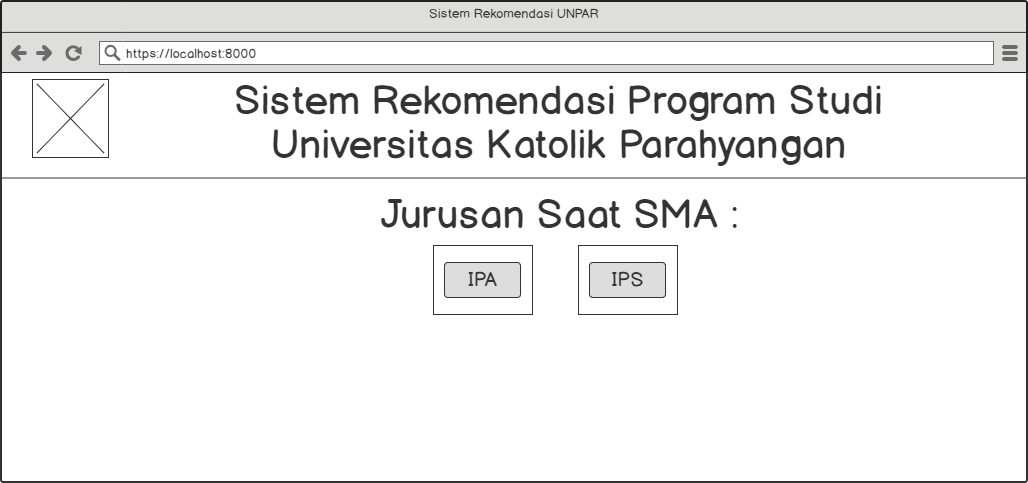
\includegraphics[width = 12cm, height =8 cm]{Gambar/gambar41.png}
        \caption{Halaman Index Sistem}
        \label{fig:gambar41}
    \end{figure}
    
    \item Halaman pengisian nilai siswa/i IPA
    
    \begin{figure}[H]
        \centering
        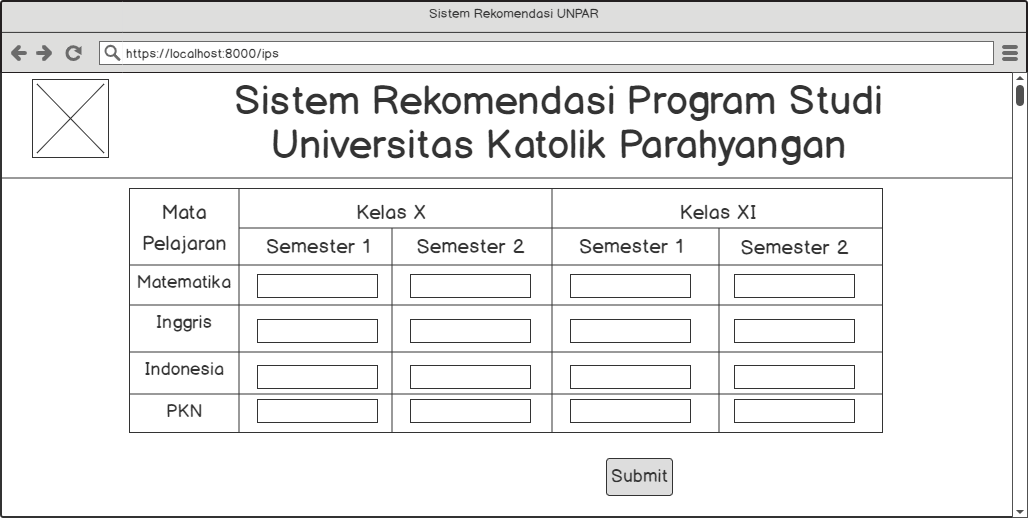
\includegraphics[width = 12cm, height =8 cm]{Gambar/gambar42.png}
        \caption{Halaman Pengisian Nilai IPA}
        \label{fig:gambar42}
    \end{figure}
    
    \item Halaman pengisian nilai siswa/i IPS
    
    \begin{figure}[H]
        \centering
        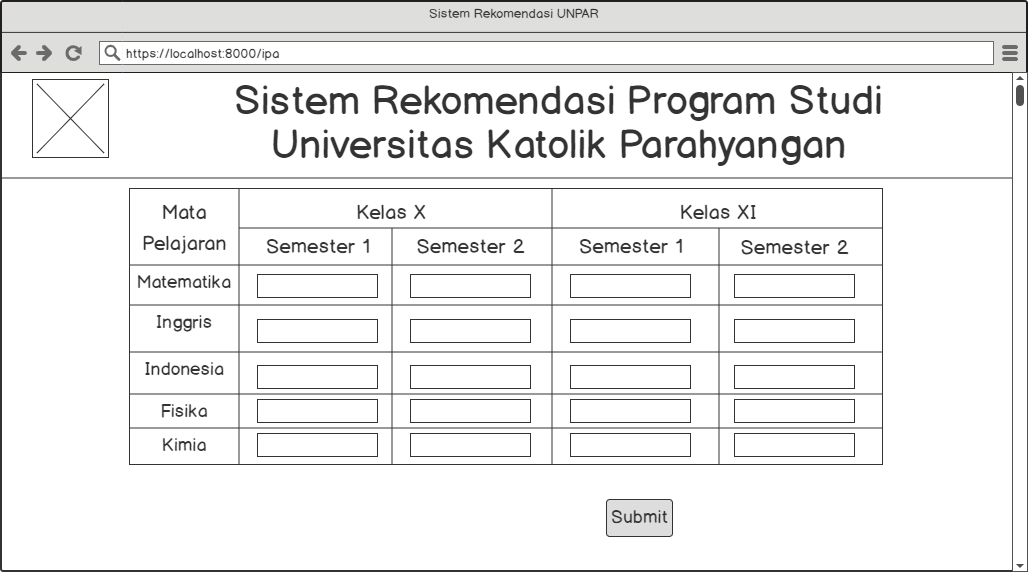
\includegraphics[width = 12cm, height =8 cm]{Gambar/gambar43.png}
        \caption{Halaman Pengisian Nilai IPS}
        \label{fig:gambar43}
    \end{figure}
    
    \item Halaman hasil rekomendasi
    
    \begin{figure}[H]
        \centering
        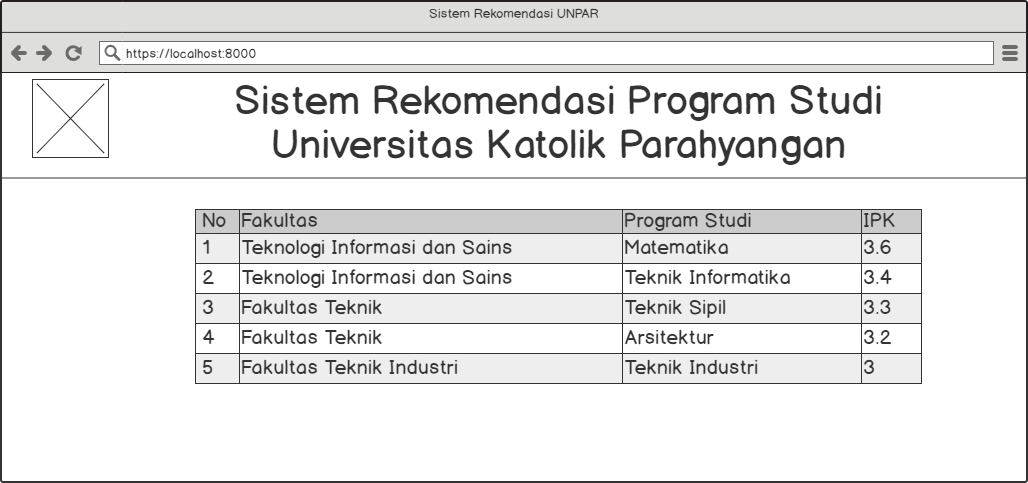
\includegraphics[width = 12cm, height =8 cm]{Gambar/gambar44.png}
        \caption{Halaman Hasil Rekomendasi}
        \label{fig:gambar44}
    \end{figure}
\end{enumerate}

\section{Perancangan Algoritma}
\label{sec:perancangan algoritma}

Pada subab ini akan berisikan perancangan algoritma yang digukan pada sistem. Sistem menggunakan beberapa algoritma seperti K-Means untuk membuat kelompok mahasiswa yang memiliki karakteriksi yang sama dengan calon mahasiswa, Pearson Correlation Coefficient untuk menghitung kemiripan, dan User-base Collaborative Filtering untuk menghitung prediksi nilai IPK.

\subsection{Preprocessing Data}
\label{subsec:perancangan preprocessing data}

Pada fungsi \textit{generateCSV} terdapat tiga \textit{parameter} \textit{mhs}, \textit{nilai}, dan \textit{count}. Parameter \textit{mhs} dan \textit{nilai} merupakan \textit{dataframe} untuk menyimpan data mahasiswa dan nilai setelah diproses, sedangkan \textit{count} digunakan untuk menyatakan berapa banyak mata pelajaran yang digunakan pada program studi di setiap fakultas. Data yang digunakan merupakan data yang berisikan mahasiswa dan nilai. Fungsi ini akan digunakan untuk data mahasiswa pada satu fakultas. Berikut merupakan \textit{pseudocode} fungsi \textit{generateCSV} : 

\begin{algorithm}[H]
  \begin{algorithmic}[1]
    \Procedure{generateCSV}{mhs, nilai, count} 
        \State $size \gets banyaknya baris pada file data$
        \State $batas \gets size/(4*count)$ \Comment{4*count karena tiap satu mata pelajaran 4 semester}
        
        \State $ipa \gets 1$ \Comment{kode jurusan ipa}
        \State $ips \gets 2$ \Comment{kode jurusan ips}
        
        \State $idUser \gets idUser saat ini$
        \State $idNilai \gets idNiali saat ini$
        
        \For{idx into batas}
            \State $idx \gets idx*(4*count)$
            \State $npm \gets NPM dari data$
            \State $idProdi \gets id prodi dari data$
            \State $isJurusan \gets ipa atau ips$ \Comment{tergantung jurusan asal}
            
            \For{i = 7 into 18}
                \State $ipk \gets ambil nilai IPK dari data$ \Comment{ambil ipk yang terakhir}
            \EndFor
            
            \State insert idUser, npm, ipk, idJurusan, dan idProdi kedalam dataframe mhs
            
            \For{i = 0 into count}
                \State $row \gets idx+i$
                \State $idMP \gets id mata pelajaran dari data$
                
                \State $m_101 \gets (nilai/20)-1$ \Comment{nilai semester 1 kelas X}
                \State $m_102 \gets (nilai/20)-1$ \Comment{nilai semester 2 kelas X}
                \State $m_111 \gets (nilai/20)-1$ \Comment{nilai semester 1 kelas XI}
                \State $m_112 \gets (nilai/20)-1$ \Comment{nilai semester 2 kelas XI}
                
                \State $avg \gets (m_101+m_102+m_111+m_112)/4$
                
                \State insert idNilai, idMP, idUser, m\_101, m\_102, m\_111, m\_112, dan avg
                
                \State $idNilai \gets idNilai+1$
            \EndFor
            \State $idUser \gets idUser+1$
        \EndFor
        \State \Return mhs, nilai
    \EndProcedure
    \State save mhs menjadi .csv
    \State save nilai menjadi .csv
  \end{algorithmic} 
  \caption{Generate CSV}
  \label{alg:generateCSV}
\end{algorithm}

\subsection{Mahasiswa Controller}
\label{subsec:mahasiswa controller}

\textit{Mahasiswa controller} berfungsi untuk mendapatkan data mahasiswa dari model \textit{MahasiswaModel}, berikut merupakan \textit{pseudocode} fungsi yang terdapat pada mahasiswa controller : \\

\begin{enumerate}
    \item Fungsi index \\
        \begin{algorithm}[H]
          \begin{algorithmic}[1]
            \Procedure{indek}{$jurusanSMA$} 
                \State $idJurusan \gets 1$ \Comment{IdJurusan IPA}
                \If{jurusanSMA == 'IPS'}
                    \State $idJurusan \gets 2$
                \EndIf
                
                \State $dataMahasiswa \gets DATAMAHASISWA(idJurusan)$
                
                \State \Return dataMahasiswa
            \EndProcedure
          \end{algorithmic} 
          \caption{Index}
          \label{alg:index mahasiswa controller}
        \end{algorithm}
        
    \item Fungsi data mahasiswa \\
        \begin{algorithm}[H]
          \begin{algorithmic}[1]
            \Procedure{dataMahasiswa}{$idJurusan$} 
                \State $query \gets$ SELECT * FROM mahasiswa INNER JOIN nilai ON mahasiswa.id\_mahasiswa = nilai.id\_mahasiswa WHERE id\_jurusan = idJurusan
                
                \State \Return query
            \EndProcedure
          \end{algorithmic} 
          \caption{Data Mahasiswa}
          \label{alg:data mahasiswa controller}
        \end{algorithm}
\end{enumerate}



\subsection{Siswa Controller}
\label{subsec:siswa controller}

\textit{Siswa controller} berfungsi untuk memproses data yang diisi oleh siswa pada gambar \ref{fig:gambar42}. Pada siswa controller terdapat atribut berupa \textit{array} yang berisikan kode mata pelajaran dan id mata pelajaran, berikut merupakan \textit{pseudocode} fungsi yang terdapat pada siswa controller :

\begin{enumerate}
    \item Fungsi index \\
        Fungsi ini digunakan untuk menerima nilai yang diisi oleh siswa, mendapatkan data mahasiswa sesuai jurusan siswa, memilih \textit{cluster} mahasiswa yang paling mirip dengan data siswa, memproses data untuk dihitung kesamaan dan prediksi, dan menampilkan pada halaman \ref{fig:gambar44}. \\
        
        \begin{algorithm}[H]
          \begin{algorithmic}[1]
            \Procedure{index}{$request$} 
                \State $data \gets request.INPUT()$
                \State $DATASISWA(data)$
                
                \State $mahasiswa \gets MAHASISWACONTROLLER()$
                \State $mhs \gets mahasiswa.INDEX(siswa["btn"]).TOARRAY()$
                
                \State $kmeans \gets KMEANSCONTROLLER(k, mhs)$ \Comment{k adalah jumlah kelompok yang ingin dibentuk}
                \State $cluster \gets kmeans.HITUNGJARAKSISWA(siswa)$
                
                \State $mhs \gets kmeans.GETCLUSTER(cluster)$
                
                \State $userBasedModel \gets USERBASEDMODELCONTROLLER(mhs, siswa)$
                
                \State $result \gets userBasedModel.GETRESULT()$
                
                \State \Return $view('/result', ['result' \gets result])$
            \EndProcedure
          \end{algorithmic} 
          \caption{Index}
          \label{alg:index siswa controller}
        \end{algorithm}

    \item Fungsi data siswa \\
        Fungsi ini digunakan untuk memproses data yang diinput oleh siswa agar format yang disimpan pada \textit{array} sama seperti data mahasiswa.\\
        
        \begin{algorithm}[H]
          \begin{algorithmic}[1]
            \Procedure{dataSiswa}{$data$} 
                \State $i \gets 1$
                \State $result \gets ARRAY()$
                \State $result['nilai'] \gets ARRAY()$
                
                \ForEach{$key => value \in data$}
                    \If{key == '\_token'}
                        \State $result[key] \gets value$
                    \Else
                        \If{i == 1}
                            \State $k \gets SUBSTR(key, 0, 3)$
                            \State $temp \gets ARRAY()$
                            
                            \State ARRAY\_PUSH(temp, ((int)value/20)-1) \Comment{Conver kedalam GPA}
                            
                            \State $i \gets i+1$
                        \Else
                            \State ARRAY\_PUSH(temp, ((int)value/20)-1) \Comment{Conver kedalam GPA}
                            
                            \State $i \gets i+1$
                            
                            \If{i == 5}
                                \State $avg \gets ARRAY\_SUM(temp)/COUNT(temp)$
                                \State ARRAY\_PUSH(temp, avg)
                                
                                \State $temp \gets REPLACEKEY(temp, 5, 'id\_mata\_pelajaran')$
                                
                                \State ARRAY\_PUSH(result['nilai',temp)
                                
                                \State $i \gets 1$
                            \EndIf
                        \EndIf
                    \EndIf
                \EndFor
                
                \If{!EMPTY(data['btnIPA'])}
                    \State $result['btn'] \gets 'IPA'$
                \ElsIf{!EMPTY(data['btnIPS'])}
                    \State $result['btn'] \gets 'IPS'$
                \EndIf
                
                \State \Return result
            \EndProcedure
            \end{algorithmic} 
            \caption{Data Siswa}
            \label{alg:data siswa controller}
        \end{algorithm}
    
    \item Fungsi replace key
        \begin{algorithm}[H]
            \begin{algorithmic}[1]
                \Procedure{ReplaceKey}{$temp, oldKey, newKey$} 
                    \State $temp[newKey] \gets temp[oldKey]$
                    \State UNSET(temp[oldKey])
                    
                    \State \Return temp
                \EndProcedure
            \end{algorithmic} 
            \caption{Replace Key}
            \label{alg:Replace Key siswa controller}
        \end{algorithm}
\end{enumerate}

\subsection{K-Means Controller}
\label{subsec:kmeans}

\textit{K-Means controller} berfungsi untuk membuat \textit{cluster} pada data mahasiswa, agar pada saat menghitung kesamaan atau similiritas menghilangkan mahasiswa yang memiliki nilai kemiripan negatif. Pada k-means controller terdapat beberapa atribut yang digunakan, yaitu : 
\begin{enumerate}
    \item \textit{currCentroid}, untuk menyimpan \textit{centroid} saat ini.
    
    \item \textit{preCentroid}, untuk menyimpan \textit{centroid} sebelumnya.
    
    \item \textit{k}, jumlah \textit{cluster} yang akan dibuat.
    
    \item \textit{cluster}, \textit{array} untuk menyimpan anggota tiap \textit{cluster}.
    
    \item \textit{mahasiswa}, untuk menyimpan data mahasiswa yang akan dibuat \textit{cluster}.
    
    \item \textit{J0}, inisialisasi jarak total dari objek ke \textit{centroid}-nya, berisi nilai 100 pada saat awal.
    
    \item \textit{J1}, inisialisasi jarak total dari objek ke \textit{centroid}-nya, untuk centroid saat ini.
\end{enumerate}

Berikut merupkan \textit{pseudocode} fungsi yang terdapat pada \textit{k-means contrller} :

\begin{enumerate}
    \item Fungsi \textit{contruct} \\
    
        \begin{algorithm}[H]
            \begin{algorithmic}[1]
                \Procedure{Contruct}{$k, dataMahasiswa$} 
                    \State $k \gets k$
                    \State $mahasiswa \gets dataMahasiswa$
                    \State $INISIALISASICLUSTER()$
                    \State $currCentroid \gets ARRAY()$ \Comment{centroid saat ini}
                    
                    \State $J0 \gets 100$ \Comment{J0 = inisialisasi jarak total dari objek ke centroid-nya}
                    
                    \State $PILIHCENTROID()$
                    
                    \State $HITUNGJARAKMHS()$
                    
                    \State $status \gets TRUE$
                    \State $ idx \gets 0$
                    \While{status}
                        \State HITUNGCENTROIDBARU()
                        \State $idx \gets idx + 1$
                        \State $status \gets CEKBATAS()$
                        \State $HITUNGJARAKMHS()$
                    \EndWhile
                \EndProcedure
            \end{algorithmic} 
            \caption{Contruct KMeans}
            \label{alg:Contruct kmeans}
        \end{algorithm}

    
    \item Fungsi inisialisasi \textit{cluster} \\
        Inisialsai untuk atribut \textit{cluster} ke 1 sampai \textit{k}. \\
        
        \begin{algorithm}[H]
            \begin{algorithmic}[1]
                \Procedure{inisialisasiCluster}{} 
                    \State $cluster \gets ARRAY()$
                    \For{i = 1 into k}
                        \State $cluster[i] \gets ARRAY()$
                    \EndFor
                \EndProcedure
            \end{algorithmic} 
            \caption{Inisialisasi Cluster}
            \label{alg:inisialisasi cluster}
        \end{algorithm}
        
    \item Fungsi pilih \textit{centroid} \\
        Fungsi untuk memilih centroid awal pada saat \textit{k-means controller} di jalankan.\\
        
        \begin{algorithm}[H]
            \begin{algorithmic}[1]
                \Procedure{pilihCentroid}{} 
                    \State $i \gets 0$
                    \While{i < k}
                        \State $key \gets RAND(0,1739)$ \Comment{Random sebanyak jumlah mahasiswa}
                        
                        \If{check key in mahasiswa == TRUE}
                            \If{check key in mahasiswa == FALSE}
                                \State ARRAY\_PUSH(currCentroid, mahasiswa[key])
                                \State $i \gets i+1$
                            \EndIf
                        \EndIf
                    \EndWhile
                \EndProcedure
            \end{algorithmic} 
            \caption{Pilih Centroid}
            \label{alg:pilih centroid}
        \end{algorithm}
    
    \item Fungsi hitung jarak mahasiswa \\
        Menhitung jarak mahasiswa dengan \textit{centroid} dan menambahkan mahasiswa sesuai dengan jarak terpendek dengan \textit{cluster}.\\
        
        \begin{algorithm}[H]
            \begin{algorithmic}[1]
                \Procedure{hitungJarakMhs}{} 
                    \State $J1 \gets 0$
                    
                    \ForEach{$valueMhs \in mahasiswa$}
                        \State $temoCluster \gets ARRAY()$ \Comment{Penampung cluster sementara}
                        \State $nilaiMhs \gets valueMhs['nilai']$
                        
                        \ForEach{$valueNilaiMhs \in nilaiMhs$}
                            \State $arrayJarak \gets ARRAY()$
                            
                            \ForEach{$valueNilaiCen \in currCentroid$}
                                \If{$(valueNilaiMhs['id_mata_pelajaran'] == 1 AND valueNilaiCen['id_mata_pelajaran'] == 1) OR (valueNilaiMhs['id_mata_pelajaran'] == 3 AND valueNilaiCen['id_mata_pelajaran'] == 3)$}
                                    \State $jarak \gets EUCLIDEANCEDISTANCE(valueNilaiMhs, valueNilaiCen)$
                                \ElsIf{$valueNilaiMhs['id_mata_pelajaran'] < valueNilaiCen['id_mata_pelajaran']$}
                                    \State break
                                \EndIf
                            \EndFor
                            \State ARRAY\_PUSH(arrJarak, jarak)
                        \EndFor
                        
                        \If{$tempCluster is empty$}
                            \State ARRAY\_PUSH(tempCluster, arrJarak)
                        \Else
                            \For{i = 1 into k}
                                \State $tempCluster[0][i] \gets tempCluster[0][i]+ arrJarak[i]$
                                \State $tempCluster[0][i] \gets SQRT(tempCluster[0][i])$
                            \EndFor
                        \EndIf
                        
                        \State $c \gets current mahasiswa cluster$
                        \State $J1 \gets J1 + tempCluster[0][c]$
                        \State ARRAY\_PUSH(tempCluster[0], c, valueMhs['id\_mahasiswa'])
                        
                        \State $tempCluster[0]['id\_mahasiswa'] \gets tempCluster[0][k+1]$
                        \State UNSET(tempCluster[0][k+1])
                        
                        \State ARRAY\_PUSH(cluster[c],valueMhs)
                    \EndFor
                \EndProcedure
            \end{algorithmic} 
            \caption{Hitung Jarak Mahasiswa}
            \label{alg:hitungJarakMhs}
        \end{algorithm}
    
    \item Fungsi hitung jarak siswa \\
        Menghitung jarak siswa dengan \textit{centroid} dan mengembalikan nomor \textit{cluster} yang paling mirip dengan siswa.\\
        
        \begin{algorithm}[H]
            \begin{algorithmic}[1]
                \Procedure{hitungJarakSiswa}{siswa} 
                    \State $nilaiSiswa \gets siswa['nilai']$
                    \State $tempCluster \gets ARRAY()$
                    
                    \ForEach{$valueNilaiSiswa \in nilaiSiswa$}
                        \State $arrJarak \gets ARRAY()$
                        
                        \ForEach{$valueCen \in currCentroid$}
                            \State $jarak \gets 0$
                            \State $nilaiCen \gets valueCen['nilai']$
                            
                            \ForEach{$valueNilaiCen \in nilaiCen$}
                                \If{$(valueNilaiMhs['id_mata_pelajaran'] == 1 AND valueNilaiCen['id_mata_pelajaran'] == 1) OR (valueNilaiMhs['id_mata_pelajaran'] == 3 AND valueNilaiCen['id_mata_pelajaran'] == 3)$}
                                \State $jarak \gets EUCLIDEANCEDISTANCE(valueNilaiSiswa, valueNilaiCen)$
                                \ElsIf{$valueNilaiMhs['id_mata_pelajaran'] < valueNilaiCen['id_mata_pelajaran']$}
                                    \State break
                                \EndIf
                            \EndFor
                            \State ARRAY\_PUSH(arrJarak,jarak)
                        \EndFor
                        \If{$tempCluster is empty$}
                            \State ARRAY\_PUSH(tempCluster, arrJarak)
                        \Else
                            \For{i = 1 into k}
                                \State $tempCluster[0][i] \gets tempCluster[0][i]+ arrJarak[i]$
                                \State $tempCluster[0][i] \gets SQRT(tempCluster[0][i])$
                            \EndFor
                        \EndIf
                    \EndFor
                    
                    \State $res \gets current siswa cluster$
                    
                    \State \Return res
                \EndProcedure
            \end{algorithmic} 
            \caption{Hitung Jarak Siswa}
            \label{alg:hitungJarakSiswa}
        \end{algorithm}
    
    \item Fungsi \textit{euclideance distance} \\
        Fungsi untuk menghitung jarak mahasiswa atau siswa dengan \textit{centroid} menggunakan metode \textit{euclideance distance}.\\
        
        \begin{algorithm}[H]
            \begin{algorithmic}[1]
                \Procedure{euclideanceDistance}{mhs, centroid} 
                    \State $result \gets 0$
                    
                    \For{i = 1 into 4}
                        \State $result \gets result + POW(mhs[i]-centroid[i],2)$
                    \EndFor
                    \State $result \gets result + POW(mhs['AVG']-centroid['AVG'],2)$
                    
                    \State \Return result
                \EndProcedure
            \end{algorithmic} 
            \caption{Euclideance Distance}
            \label{alg:euclideanceDistance}
        \end{algorithm}
    
    \item Fungsi hitung \textit{centroid} baru \\
        Fungsi untuk menghitung centroid baru dari \textit{cluster} yang sudah dibuat. \\
        
        \begin{algorithm}[H]
            \begin{algorithmic}[1]
                \Procedure{hitungCentroidBaru}{} 
                    \State $prevCentroid \gets currCentroid$
                    \State RESETCENTROID()
                    
                    \ForEach{$keyCen=>valueCen \in currCentroid$}
                        \State $nilaiCen \gets valueCen['nilai']$
                        
                        \ForEach{$keyNilaiCen=>valueNilaiCen \in nilaiCen$}
                            \State $anggota \gets cluster[keyCen]$
                            \If{numbers of anggota != 0}
                                \ForEach{$keyAnggota=>valueAnggota \in anggota$}
                                    \State $nilaiAnggota = valueAnggota['nilai']$
                                    
                                    \ForEach{$keyNilaiAnggota=>valueNilaiAnggota \in nilaiAnggota$}
                                        \If{$(valueNilaiMhs['id_mata_pelajaran'] == 1 AND valueNilaiCen['id_mata_pelajaran'] == 1) OR (valueNilaiMhs['id_mata_pelajaran'] == 3 AND valueNilaiCen['id_mata_pelajaran'] == 3)$}
                                            \For{i = 1 into 4}
                                                \State $nilaiLama \gets currCentroid[keyCen]['nilai][keyNilaiCen][i]$
                                                \State $nilaiBaru \gets anggora[keyAnggota]['nilai'][keyNilaiAnggota][i]$
                                                
                                                \State UPDATENILAI(keyCen, keyNilaiCen, nilaiLama, nilaiBaru, i)
                                            \EndFor
                                            \State $nilaiLama \gets currCentroid[keyCen]['nilai][keyNilaiCen]['AVG']$
                                            \State $nilaiBaru \gets anggora[keyAnggota]['nilai'][keyNilaiAnggota]['AVG']$
                                            \State UPDATENILAI(keyCen, keyNilaiCen, nilaiLama, nilaiBaru, 'AVG')
                                        \EndIf
                                    \EndFor
                                \EndFor
                                \Else
                                    \State RANDOMNILAIBARU(keyCen, KeyNilaiCen)
                            \EndIf
                        \EndFor
                    \EndFor
                    \State HITUNGRATA2()
                \EndProcedure
            \end{algorithmic} 
            \caption{Hitung Centroid Baru}
            \label{alg:hitungCentroidBaru}
        \end{algorithm}
        
    \item Fungsi reset \textit{centroid} \\
        
        \begin{algorithm}[H]
            \begin{algorithmic}[1]
                \Procedure{resetCentroid}{} 
                    \ForEach{$keyCen => valueCen \in currCentroid$}
                        \State $nilaiCen \gets valueCen['nilai']$
                        
                        \ForEach{$keyNilai \in nilaiCen$}
                            \For{i = 1 into 4}
                                \State $currCentroid[keyCen]['nilai'][keyNilaiCen][i] \gets 0$
                            \EndFor
                            \State $currCentroid[keyCen]['nilai'][keyNilaiCen]['AVG'] \gets 0$
                        \EndFor
                    \EndFor
                \EndProcedure
            \end{algorithmic} 
            \caption{Reset Centroid}
            \label{alg:resetCentroid}
        \end{algorithm}
        
    \item Fungsi \textit{update} nilai \\
        Fungsi untuk \textit{update} nilai \textit{centroid} baru.\\
        
        \begin{algorithm}[H]
            \begin{algorithmic}[1]
                \Procedure{updateNilai}{keyCen, keyNilaiCen, nilaiLama, nilaiBaru, i} 
                  \State $nilai \gets nilaiLama+nilaiBaru$
                  \State $currCentroid[keyCen]['nilai'][keyNilaiCen][i] \gets nilai$
                \EndProcedure
            \end{algorithmic} 
            \caption{Update Nilai}
            \label{alg:updateNilai}
        \end{algorithm}
        
    \item Fungsi hitung rata-rata \\
        Fungsi untuk menghitung rata-rata nilai yang sudah di-\textit{update}.\\
        
        \begin{algorithm}[H]
            \begin{algorithmic}[1]
                \Procedure{hitungRata2}{} 
                    \ForEach{$keyCen => valueCen \in currCentroid$}
                        \State $nilaiCen \gets valueCen['nilai']$
                        \State $anggota \gets cluster[keyCen]$
                        \State $count \gets numbers of anggota$
                        \If{counter != 0}
                            \ForEach{$keyNilaiCen \in nilaiCen$}
                                \For{i = 1 into 4}
                                    \State $currCentroid[keyCen]['nilai'][keyNilaiCen][i] \gets currCentroid[keyCen]['nilai'][keyNilaiCen][i]/count$
                                \EndFor
                                $currCentroid[keyCen]['nilai'][keyNilaiCen]['AVG'] \gets currCentroid[keyCen]['nilai'][keyNilaiCen]['AVG']/count$
                            \EndFor
                        \EndIf
                    \EndFor
                \EndProcedure
            \end{algorithmic} 
            \caption{Hitung Rata2}
            \label{alg:hitungRata2}
        \end{algorithm}
    
    \item Fungsi \textit{random} nilai baru \\
    
        Fungsi untuk \textit{random} nilai baru, jika tidak terdapat anggota pada suatu \textit{cluster}. \\
        
        \begin{algorithm}[H]
            \begin{algorithmic}[1]
                \Procedure{randomNilaiBaru}{keyCen, keyNilaiCen} 
                    \For{i = 1 into 4}
                        \State $currCentroid[keyCen]['nilai'][keyNilaiCen][i] \gets RAND(1,3) + RAND(1,10)/10$
                    \EndFor
                     \State $currCentroid[keyCen]['nilai'][keyNilaiCen]['AVG'] \gets RAND(1,3) + RAND(1,10)/10$
                \EndProcedure
            \end{algorithmic} 
            \caption{Random NilaiBaru}
            \label{alg:randomNilaiBaru}
        \end{algorithm}
    
    \item Fungsi cek batas \\
    
        Fungsi untuk mengecek apakah batas < 0.01, jika iya berarti anggota pada suatu \textit{cluster} sudah konvergen. \\
        
        \begin{algorithm}[H]
            \begin{algorithmic}[1]
                \Procedure{cekBatas}{} 
                    \State $batas \gets ABS(J0 - J1)$
                    
                    \If{batas < 0.1}
                        \State \Return FALSE
                    \EndIf
                    
                    \State \Return TRUE
                \EndProcedure
            \end{algorithmic} 
            \caption{Cek Batas}
            \label{alg:cekBatas}
        \end{algorithm}
        
    \item Fungsi \textit{get cluster} \\
    
        Fungsi untuk mendapatkan \textit{cluster} yang sesuai dengan \textit{cluster} yang sudah dibentuk.\\
        
        \begin{algorithm}[H]
            \begin{algorithmic}[1]
                \Procedure{getCluster}{idx} 
                    \State \Return cluster[idx]
                \EndProcedure
            \end{algorithmic} 
            \caption{Get Cluster}
            \label{alg:getCluster}
        \end{algorithm}
    
\end{enumerate}

\subsection{User Based Model Controller}
\label{subsec:user-based}

\textit{User Based Model Controller} berfungsi untuk mengidentifikasi pengguna yang akan diberikan rekomendasi dengan pengguna lain. Terdapat tiga atribut pada \textit{user base model controller} yaitu :

\begin{enumerate}
    \item \textit{pearsonCorrelation}, untuk menampung \textit{PearsonController}.
    
    \item \textit{prediction}, untuk menampung \textit{PredictionController}.
    
    \item \textit{result}, untuk menampung hasil prediksi.
\end{enumerate}

Berikut merupakan \textit{pseudocode} fungsi yang terdapat pada \textit{user based model controller} : 

\begin{enumerate}
    \item Fungsi \textit{contruct} \\
        
        Terdapat tiga parameter, yaitu : \textit{mahasiswa}, \textit{siswa}, dan \textit{mode} dengan nilai awal 0. Parameter \textit{mahasiswa} merupakan \textit{array} yang berisikan data mahasiswa, \textit{siswa} merupakan \textit{array} yang berisikan nilai siswa, dan \textit{mode} merupakan mode yang digunakan pada saat \textit{user based model controller} dijalankan, jika mode bernilai 0 berarti dalam mode penggunaan siswa dan 1 jika dalam pengujian. \\ 
        
        \begin{algorithm}[H]
            \begin{algorithmic}[1]
                \Procedure{Contruct}{$mahasiswa, siswa, mode = 0$} 
                    \State $prediction \gets PREDICTIONCONTROLLER()$
                    \If {mode == 0}
                        \State $pearsonCorrelation \gets PEARSONCORRELATIONCONTROLLER()$
                        \State $pearson \gets CALCULATESIMILARITY (mahasiswa, siswa)$
                        \State $result \gets CALCULATEPREDICT(pearson)$
                    \ElsIf {mode == 1}
                        \State $pearsonCorrelation \gets PEARSONCORRELATIONPENGUJIANCONTROLLER()$
                    \EndIf
                \EndProcedure
            \end{algorithmic} 
            \caption{Contruct}
            \label{alg:Contruct user-based}
        \end{algorithm}

    \item Fungsi \textit{calculate similarity}\\
    
        \begin{algorithm}[H]
            \begin{algorithmic}[1]
                \Procedure{calculateSimilarity}{$mahasiswa, siswa$} 
                    \State \Return $pearsonCorrelation \gets CALCULATEPEARSON(mahaiswa, siswa)$
                \EndProcedure
            \end{algorithmic} 
            \caption{Calculate Similarity}
            \label{alg:calculateSimilarity}
        \end{algorithm}
    
    \item Fungsi \textit{calculate prediction}\\
        
        \begin{algorithm}[H]
            \begin{algorithmic}[1]
                \Procedure{calculatePredict}{$pearson$} 
                    \State \Return $prediction \gets CALCULATEPREDICT(pearson)$
                \EndProcedure
            \end{algorithmic} 
            \caption{Calculate Predict}
            \label{alg:calculatePredict}
        \end{algorithm}
        
    \item Fungsi \textit{get result}\\
        
        \begin{algorithm}[H]
            \begin{algorithmic}[1]
                \Procedure{getResult}{} 
                    \State \Return result
                \EndProcedure
            \end{algorithmic} 
            \caption{User-based Collaborative Filtering}
            \label{alg:getResult user-based}
        \end{algorithm}
    
\end{enumerate}

\subsection{Pearson Correlation Controller}
\label{subsec:pearson}

\textit{Pearson correlation controller} berfungsi untuk menghitung kesamaan pengguna dengan pengguna lain, berikut merupakan \textit{pseudocode} fungsi yang terdapat pada \textit{pearson correlation controller} :

\begin{enumerate}
    \item Fungsi \textit{calcaulate pearson}\\
    
        \begin{algorithm}[H]
            \begin{algorithmic}[1]
                \Procedure{calculatePearson}{$mahasiswa, siswa$} 
                    \State $res \gets ARRAY()$
                    \ForEach{$mhs \in mahasiswa$}
                        \State $covariance \gets CALCULATECOVARIANCE(mhs, siswa)$
                        \State $sd \gets CALCULATESTANDARDEVIATION(mhs,siswa)$
                        \State $sdMhs \gets sd[0]$
                        \State $sdSiswa \gets sd[1]$
                        
                        \State $idProdi \gets mhs['id_program\_studi']$
                        \State $IPK \gets mhs['IPK']$
                        
                        \State $sim \gets CONVARIANCE / (sdMhs * sdSiswa)$
                        
                        \If{$sim > 0$}
                            \State $res[mhs['id\_mahasiswa']] \gets ARRAY()$
                            \State $ARRAY\_PUSH(res[mhs['id\_mahasiswa']], sim, idProdi, IPK)$
                        \EndIf
                    \EndFor
                
                    \State \Return res
                \EndProcedure
            \end{algorithmic} 
            \caption{Calculate Pearson}
            \label{alg:calculatePearson}
        \end{algorithm}
        
    \item Fungsi \textit{calculate covaraiance}\\
        
        \begin{algorithm}[H]
            \begin{algorithmic}[1]
                \Procedure{calculateCovariance}{$mhs, siswa$} 
                    \State $res \gets 0$
                    \State $nilaiMhs \gets mhs['nilai']$
                    \State $nilaiSiswa \gets siswa['nilai']$
                    
                    \ForEach{$nSiswa \in nilaiSiswa$}
                        \State $idMP \gets nSiswa['id\_mata\_pelajaran']$
                        \ForEach{$nMhs \in nilaiMhs$}
                            \If{idMP == nMhs['id\_mata\_pelajaran']}
                                \For{i = 1 to 4}
                                    \State $res \gets res +  (nMhs[i]-nMhs['AVG'])*(nSiswa[i]-nSiswa['AVG'])$
                                \EndFor
                            \ElsIf{idMP < nMhs['id\_mata\_pelajaran']}
                                \State break
                            \EndIf
                        \EndFor
                    \EndFor
                    \State \Return res
                \EndProcedure
            \end{algorithmic} 
            \caption{Calculate Covariance}
            \label{alg:calculateCovariance}
        \end{algorithm}
        
    \item Fungsi \textit{calculate standar deviation}\\
        
        \begin{algorithm}[H]
            \begin{algorithmic}[1]
                \Procedure{calculateStandarDeviation}{$mhs, siswa$} 
                    \State $res \gets 0$
                    
                    \State $sdMhs \gets 0$
                    \State $sdSiswa \gets 0$
                    
                    \State $nilaiMhs \gets mhs['nilai']$
                    \State $nilaiSiswa \gets siswa['nilai']$
                    
                    \ForEach{$nSiswa \in nilaiSiswa$}
                        \State $idMP \gets nSiswa['id\_mata\_pelajaran']$
                        \ForEach{$nMhs \in nilaiMhs$}
                            \If{idMP == nMhs['id\_mata\_pelajaran']}
                                \For{i = 1 to 4}
                                    \State $sdMhs \gets sdMhs + POW(nMhs[i]-nMhs['AVG'],2)$
                                    \State $sdSiswa \gets sdSiswa + POW(nSiswa[i]-nSiswa['AVG'],2)$
                                \EndFor
                            \ElsIf{idMP < nMhs['id\_mata\_pelajaran']}
                                \State break
                            \EndIf
                        \EndFor
                    \EndFor
                    \State $ARRAY\_PUSH(res, SQRT(sdMhs), SQRT(sdSiswa))$
                    
                    \State \Return res
                \EndProcedure
            \end{algorithmic} 
            \caption{Calculate Standar Deviation}
            \label{alg:calculateStandarDeviation pearson}
        \end{algorithm}
\end{enumerate}

\subsection{Precidtion Controller}
\label{subsec:prediction}

\textit{Prediction controller} berfungsi untuk menghitung prediksi dari hasil perhitungan kemiripan menggunkan \textit{pearson correlation}. Terdapat dua atribut dalam \textit{prediction controller}, yaitu :

\begin{enumerate}
    \item \textit{programStudi}, untuk menyimpan \textit{ProgramStudiController}.
    
    \item \textit{fakultas}, untuk menyimpan \textit{FakultasController}.
\end{enumerate}

Berikut merupakan \textit{pseudocode} fungsi yang terdapat pada \textit{prediction controller} :

\begin{enumerate}
    \item Fungsi \textit{contruct}\\
    
        \begin{algorithm}[H]
            \begin{algorithmic}[1]
                \Procedure{Contruct}{} 
                    \State $programStudi \gets PROGRAMSTUDICONTROLLER()$
                    \State $fakultas \gets FAKULTASCONTROLLER()$
                \EndProcedure
            \end{algorithmic} 
            \caption{Contruct}
            \label{alg:Contruct prediction}
        \end{algorithm}

    \item Fungsi \textit{calculate predict}\\
        
        \begin{algorithm}[H]
            \begin{algorithmic}[1]
                \Procedure{calculatePredict}{$pearson$} 
                    \State $res \gets ARRAY()$
                    
                    \State $a \gets 0$ \Comment{a = Sigma(sim*IPK)}
                    \State $b \gets 0$ \Comment{b = Sigma(sim)}
                    
                    \ForEach{$id\_mhs => value \in pearson$}
                        \State $a \gets a + value[0]*value[2]$
                        \State $b \gets b + value[0]$
                        
                        \State $next \gets NEXT(pearson)$
                        
                        \If{$next != NULL$}
                            \If{$value[1] != next[1]$}  
                                \State $res \gets INSERTDATA(res, a, b, value[1])$
                                
                                \State $a \gets 0$
                                \State $b \gets 0$
                            \EndIf
                        \ElsIf{$next != NULL$}
                            \State $res \gets INSERTDATA(res, a, b, value[1])$
                        \EndIf
                    \EndFor
                    
                    \State $score \gets ARRAY_COLUMN(res,0)$ \Comment{Penampung nilai prediksi IPK}
                    \State $ARRAY\_MULTISORT(score, SORT\_DESC, res)$ \Comment{Sort berdasarkan nilai prediksi terbesar}
                    
                    \State \Return res
                \EndProcedure
            \end{algorithmic} 
            \caption{Calculate Predict}
            \label{alg:calculate Predict1}
        \end{algorithm}
    
    \item Fungsi \textit{insert data} \\

        \begin{algorithm}[H]
            \begin{algorithmic}[1]
                \Procedure{insertData}{$res, a, b, idProdi$} 
                    \State $pred \gets a/b$
                    \State $namaFakultas \gets fakultas.GETNAMAFAKULTAS(idProdi)$
                    \State $namaProdi \gets programStudi.GETNAMAPROGRAMSTUDI(idProdi)$
                    \State $res[idProdi] \gets ARRAY()$
                    \State $ARRAY\_PUSH(res[idProdi], pred, namaFakultas, namaProdi)$
                    \State \Return res
                \EndProcedure
            \end{algorithmic} 
            \caption{Insert Data}
            \label{alg:insertData prediction}
        \end{algorithm}
\end{enumerate}


\subsection{Fakultas Controller}
\label{subsec:fakultas controller}

\textit{Fakultas controller} berfungsi untuk mendapatkan data fakultas dari model \textit{FakultasModel}, berikut merupakan \textit{pseudocode} fungsi yang terdapat pada \textit{fakultas controller} :

\begin{enumerate}
    \item Fungsi \textit{get} nama fakultas \\
    
        \begin{algorithm}[H]
            \begin{algorithmic}[1]
                \Procedure{getNamaFakultas}{idProgramStudi}
                    \State $idFakultas \gets FLOOR(idProgramStudi)$
                    \State $namaFakultas \gets$ SELECT nama\_fakultas FROM fakultas WHERE idFakultas = idProgramStudi
                    
                    \State \Return namaFakultas
                \EndProcedure
            \end{algorithmic} 
            \caption{Get Nama Fakultas}
            \label{alg:getNamaFakultas}
        \end{algorithm}
\end{enumerate}


\subsection{Program Studi Controller}
\label{subsec:prodicontroller}

\textit{Program studi controller} berfungsi untuk mendapatkan data program studi dari model \textit{ProgramStudisModel}, berikut merupakan \textit{pseudocode} fungsi yang terdapat pada \textit{program studi controller} :

\begin{enumerate}
    \item Fungsi \textit{get} nama program studi \\
        
        \begin{algorithm}[H]
            \begin{algorithmic}[1]
                \Procedure{getNamaProgramStudi}{idProgramStudi} 
                    \State $namaProdi \gets$ SELECT nama\_program\_studi FROM program\_studi WHERE id\_program\_studi = idProgramStudi
                    
                    \State \Return namaProdi
                \EndProcedure
            \end{algorithmic} 
            \caption{getNamaProgramStudi}
            \label{alg:getNamaProgramStudi}
        \end{algorithm}
        
\end{enumerate}



\subsection{Pengujian Controller}
\label{subsec:pengujian controller}

\textit{Pengujian controller} digunakan untuk melakukkan pengujian terhadap sistem rekomendasi program studi Universitas Katolik Parahyangan. Pengujian dilakukan dengan menghitung akurasi dan waktu eksekusi program. Terdapat beberapa atribut pada \textit{pengujian controller}, yaitu :

\begin{enumerate}
    \item \textit{train}, untuk data \textit{train} dari hasil pembagian data.
    
    \item \textit{test}, untuk data \textit{test} dari hasil pembagian data.
    
    \item \textit{userBasedModel}, untuk menyimpan \textit{UserBaseModelController}
    
    \item \textit{error1}, untuk menyimpan selisih nilai yang akan digunakan untuk \textit{mae}.
    
    \item \textit{error2}, untuk menyimpan selisih nilai yang akan digunakan untuk \textit{rmmse}.
    
    \item \textit{accuracy}, untuk menyimpan \textit{AccuracyController}.
    
    \item \textit{metode}, untuk menyimpan metode pengujian yang digunakan.
\end{enumerate}

Berikut merupakan \textit{pseudocode} fungsi yang terdapat pada \textit{pengujian controller} :

\begin{enumerate}
    \item Fungsi \textit{contruct}\\
        
        \begin{algorithm}[H]
            \begin{algorithmic}[1]
                \Procedure{Contruct}{request} 
                   \State $btn \gets request.INPUT()$
                   \State $idJurusan \gets SUBSTR(btn['btn'], 0, 3)$
                   \State $metode = SUBSTR(btn['btn'], 4, STRLEN(btn['btn']))$
                   
                   \State $mhs \gets MAHASISWACONTROLLER()$
                   \State $data \gets mhs.INDEX(idJurusan).TOARRAY()$
                   
                   \State $arrLabel \gets ARRAY()$ \Comment{Penampung label data}
                   
                   \ForEach{$m \in data$}
                        \State ARRAY\_PUSH(arrLabel, m['id\_program\_studi']
                   \EndFor
                   
                   \State $dataSet \gets ARRAYDATASET(data, arrLabel)$
                   \State $dataset \gets RANDOMSPLIT(dataset, n)$ \Comment{n = numbers of size (0.1 - 0.9)}
                   
                   \State $train \gets dataset.GETTRAINSAMPLES$
                   \State $test \gets dataset.GETTESTSAMPLES$
                   
                   \State $accuracy \gets ACCURACYCONTROLLER()$
                   
                   \State $userBasedModel \gets USERBASEDMODELCONTROLLER(NULL, NULL, 1)$
                \EndProcedure
            \end{algorithmic} 
            \caption{Contruct}
            \label{alg:contruct pengujian}
        \end{algorithm}

    \item Fungsi index\\
        Fungsi untuk menentukan metode yang digunakan. Terdapat dua metode, yaitu : pengujian \textit{basic} atau dasar dan pengujian menggunkan metode \textit{kmeans}. \\
        
        \begin{algorithm}[H]
            \begin{algorithmic}[1]
                \Procedure{index}{} 
                   \If{metode == 'Basic'}
                        \State \Return PENGUJIANBASIC()
                   \Else
                        \State \Return PENGUJIANKMEANS(bts, n)
                   \EndIf
                \EndProcedure
            \end{algorithmic} 
            \caption{Index}
            \label{alg:index}
        \end{algorithm}
    
    \item Fungsi pengujian \textit{basic}\\
    
        \begin{algorithm}[H]
            \begin{algorithmic}[1]
                \Procedure{pengujianBasic}{} 
                   \State $result \gets ARRAY()$
                   
                   \State $error1 \gets ARRAY()$
                   \State $error2 \gets ARRAY()$
                   
                   \ForEach{$t \in test$}
                        \State $start \gets count time$
                        
                        \If{t['NPM'] NOT IN result}
                            \State $temp \gets ARRAY()$
                            
                            \State $pearson \gets userBasedModel.CALCULATESIMILARITY(train, t)$
                            
                            \State $predict \gets userBasedModel.CALCULATEPREDICT(pearson)$
                            
                            \If{predict != NULL}
                                \State $diff1 \gets ABS(t['IPK'] - predict[0][0])$
                                \State ARRAY\_PUSH(error1, diff1)
                                
                                \State $diff2 \gets POW(t['IPK'] - predict[0][0],2)$
                                \State ARRAY\_PUSH(error2, diff2)
                                
                                \State ARRAY\_PUSH(temp, t['NPM'], predict[0][2],t['IPK'], predict[0][0], diff1, diff2)
                                
                                \State ARRAY\_PUSH(result, temp)
                            \EndIf
                        \EndIf
                   \EndFor
                   
                   \State $mae \gets accuracy.CALCULATEMAE(error1)$
                   \State $rmse \gets accuracy.CALCULATERMSE(error2)$
                   \State $end \gets count time$
                   \State $times \gets end - start$
                   
                   \State \Return view('/pengujian',['status'=>TRUE, 'result'=>result, 'mae'=>mae, 'rmse'=>rmse, 'times'=>times, 'metode'=>metode])
                \EndProcedure
            \end{algorithmic} 
            \caption{Pengujian Basic}
            \label{alg:pengujianBasic}
        \end{algorithm}
    
    \item Fungsi pengujian \textit{kmeans}\\
        Pengujian menggunakan metode \textit{kmeans} terdapat dua parameter, yaitu : \textit{bts} dan \textit{n}. Parameter \textit{bts} berfungsi untuk batas k yang akan dicoba dan \textit{n} berfungsi untuk mengulang sebanyak n kali proses \textit{clustering}.
        
        \begin{algorithm}[H]
            \begin{algorithmic}[1]
                \Procedure{pengujianKmeans}{bts, n} 
                   \State $result \gets ARRAY()$
                   \State $resultPred \gets ARRAY()$
                   
                   \For{k = 2 into bts}
                        \State $start \gets count time$
                        \State $tempMae \gets 0$
                        \State $tempRmse \gets 0$
                        
                        \For{i = 1 into n}
                            \State $kmeans \gets KMEANSCOONTROLLER(k, train)$
                            
                            \State $error1 \gets ARRAY()$
                            \State $error2 \gets ARRAY()$
                            
                            \ForEach{$t \in test$}
                                \If{t['NPM'] NOT IN resultPred}
                                    \State $temp \gets ARRAY()$
                                    
                                    \State $cluster \gets kmeans.HITUNGJARAKSISWA(t)$
                                    
                                    \State $dataTrain \gets kmeans.GETCLUSTER(cluster)$
                                    
                                    \State $pearson \gets userBasedModel.CALCULATESIMILARITY(dataTrain, t)$
                                    \State $predict \gets userBasedModel.CALCULATEPREDICT(pearson)$
                                    
                                    \If{predict != NULL}
                                        \State $diff1 \gets ABS(t['IPK'] - predict[0][0])$
                                        \State ARRAY\_PUSH(error1, diff1)
                                        
                                        \State $diff2 \gets POW(t['IPK'] - predict[0][0],2)$
                                        \State ARRAY\_PUSH(error2, diff2)
                                        
                                        \State ARRAY\_PUSH(temp, t['NPM'], predict[0][2],t['IPK'], predict[0][0], diff1, diff2)
                                        
                                        \State ARRAY\_PUSH(resultPred, temp)
                                    \EndIf
                                \EndIf
                            \EndFor
                                \State $mae \gets accuracy.CALCULATEMAE(error1)$
                                \State $rmse \gets accuracy.CALCULATERMSE(error2)$
                                
                                \State $tempMae \gets tempMae + mae$
                                \State $tempRmse \gets tempRmse + rmse$
                        \EndFor
                        \State $end \gets count time$
                        \State $times \gets end - start$
                        
                        \State $result[k] \gets ARRAY()$
                        
                        \State $ARRAY_PUSH(result[k], tempMae/n, tempRmse/n, times)$
                        
                   \EndFor
                   
                   \State $minMae \gets MIN(ARRAY_COLUMN(result,0))$
                   \State $minRmse \gets MIN(ARRAY_COLUMN(result,1))$
                   \State $minTime \gets MIN(ARRAY_COLUMN(result,2))$
                   
                   \State \Return $view('/pengujian', [
                        'status' \gets TRUE, 'resultPred' \gets resultPred, 'metode' \gets metode, 'result' \gets result, 'minMae' \gets minMae, 'minRmse' => minRmse, 'minTime' \gets minTime
                    ])$
                \EndProcedure
            \end{algorithmic} 
            \caption{Pengujian Kmeans}
            \label{alg:pengujianKmeans}
        \end{algorithm}

\end{enumerate}

\subsection{Pearson Correlation Pengujian Controller}
\label{subsec:pearson pengujian}

\textit{Pearson Correlation pengujina controller} digunakan pada saat pengujian, yang membedakan dengan \textit{pearson correlation} hanya pada fungsi \textit{calculate pearson}, dimana hanya menghitung prediksi sesuai dengan program studi mahsiswa yang dicek. Berikut merupakan \textit{pseudocode} fungsi yang terdapat pada \textit{pearson correlation pengujian controller} :

\begin{enumerate}
        \item Fungsi \textit{calculaye pearson} \\
        
        \begin{algorithm}[H]
            \begin{algorithmic}[1]
                \Procedure{calculatePearson}{$mahasiswa, siswa$} 
                    \State $res \gets ARRAY()$
                    \ForEach{$mhs \in mahasiswa$}
                        \If{mhs['id\_program\_studi'] == siswa['id\_program\_studi']}
                            \State $covariance \gets CALCULATECOVARIANCE(mhs, siswa)$
                            \State $sd \gets CALCULATESTANDARDEVIATION(mhs,siswa)$
                            \State $sdMhs \gets sd[0]$
                            \State $sdSiswa \gets sd[1]$
                            
                            \State $idProdi \gets mhs['id_program\_studi']$
                            \State $IPK \gets mhs['IPK']$
                            
                            \State $sim \gets CONVARIANCE / (sdMhs * sdSiswa)$
                            
                            \If{$sim > 0$}
                                \State $res[mhs['id\_mahasiswa']] \gets ARRAY()$
                                \State $ARRAY\_PUSH(res[mhs['id\_mahasiswa']], sim, idProdi, IPK)$
                            \EndIf
                        \EndIf
                    \EndFor
                
                    \State \Return res
                \EndProcedure
            \end{algorithmic} 
            \caption{Calculate Pearson Pengujian}
            \label{alg:calculatePearsonPengujian}
        \end{algorithm}
        
        \item Fungsi \textit{calculate covariance} sama seperti \ref{alg:calculateCovariance}.
        
        \item Fungsi \textit{calculate standar deviation} sama seperti \ref{alg:calculateStandarDeviation pearson}. 
\end{enumerate}


\subsection{Accuracy Controller}
\label{subsec:accuracy}

\textit{Accuracy Controller} digunakan untuk menghitung akurasi dari sistem rekomendasi program studi Universitas Katolik Parahyangan, berikut merupakan \textit{pseudocode} fungsi yang terdapat pada \textit{accuracy controller} :

\begin{enumerate}
    \item Fungsi \textit{calculate mae}\\
    
        \begin{algorithm}[H]
            \begin{algorithmic}[1]
                \Procedure{calculateMAE}{arr} 
                   \State \Return ARRAY\_SUM(arr)/COUNT(arr)
                \EndProcedure
            \end{algorithmic} 
            \caption{Calculate MAE}
            \label{alg:calculateMAE}
        \end{algorithm}
    
    \item Fungsi \textit{calculate rmse}\\
    
        \begin{algorithm}[H]
            \begin{algorithmic}[1]
                \Procedure{calculateRMSE}{arr} 
                   \State \Return SQRT(ARRAY\_SUM(arr)/COUNT(arr))
                \EndProcedure
            \end{algorithmic} 
            \caption{Calculate RMSE}
            \label{alg:calculateRMSE}
        \end{algorithm}
\end{enumerate}

\section{Perancangan \textit{Class Diagram}}
\label{sec:perancangan class diagram}

\begin{figure}[H]
    \centering
    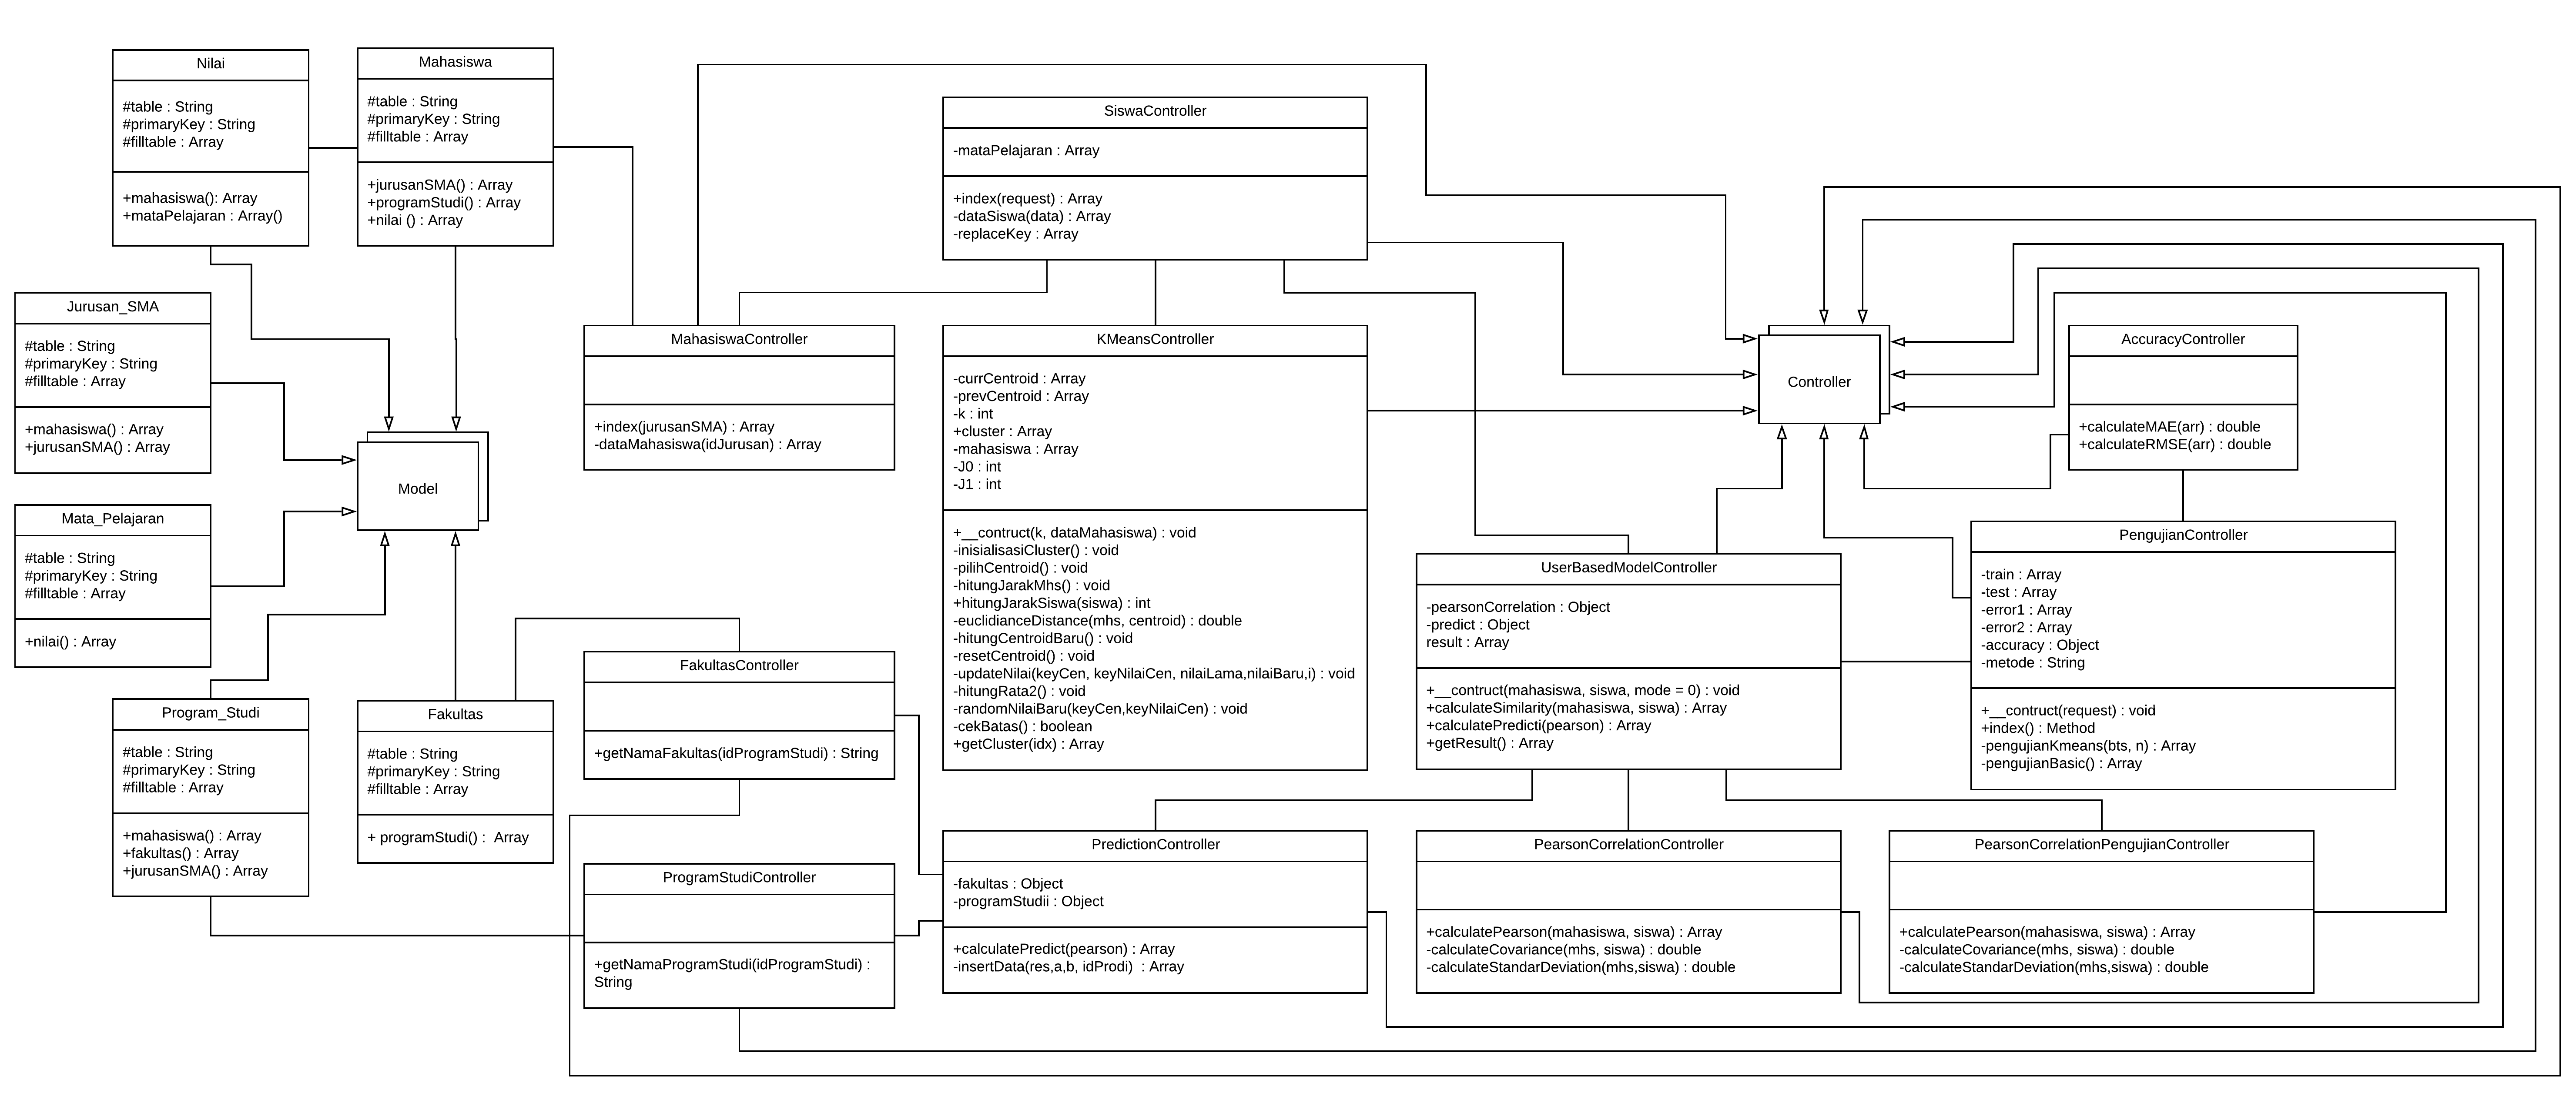
\includegraphics[width = 20cm, height = 15cm, angle = 90]{Gambar/gambar45.png}
    \caption{\textit{Class Diagram} Sistem Rekomendasi}
    \label{fig:class diagram sistem rekomendasi}
\end{figure}